%%
%% Latex Style File for MECH0020 - AY 2023/2024
%%
%% I. Eames 
%% version 2
%% 26th March 2024
%% Uses vanilla form of latex with no need to additional style files
%%

\documentclass[11pt,twocolumn]{article} 
\usepackage{fancyhdr}
\usepackage{expl3,xparse,xcoffins,titling,kantlipsum}
\ExplSyntaxOn
\coffin_new:N \l_my_abstract_coffin
\dim_zero_new:N \l_my_width_dim
\keys_define:nn { my / abstract }
  {
    width .code:n = {
      \dim_set:Nn \l_my_width_dim {#1\textwidth}
    }
  }
\NewDocumentCommand \myabstract { O {width=.8} m }{%
  \keys_set:nn { my / abstract } { #1 }
  \SetVerticalCoffin \l_my_abstract_coffin {\l_my_width_dim} {#2}
  \renewcommand\maketitlehookd{%
    \mbox{}\medskip\par
    \centering
    \TypesetCoffin \l_my_abstract_coffin
  }
}
\ExplSyntaxOff
\usepackage[document]{ragged2e}
\usepackage{geometry}
 \geometry{
  a4paper,
  total={170mm,257mm},
  left=17.5mm,
  right=17.5mm,
  bottom=15mm,
  top=15mm
 }
 
% \documentclass{gji}
\usepackage{timet,color}
\usepackage{nomencl}
\setlength{\nomitemsep}{-\parsep}
\usepackage{graphicx}
\usepackage[urlcolor=blue,citecolor=black,linkcolor=black]{hyperref}
\usepackage[english]{babel}
\usepackage{times}
\usepackage{multicol}
\usepackage{amsmath}
\usepackage{float}
\makenomenclature
\begin{document}

\title{\bf \Huge Monte Carlo Localization}
\author{{\bf Juan Alvarez, Joel Santiago-Baretti, Erica Chen, Mohammed Ehab, Ningshan Ma}\\
   RSS: Robotics, Science, and Systems \\ Team 2
  }
\date{April 8th 2024}


\let\leqslant=\leq

\label{firstpage}


%%
%% This format for begin abstract is a reclaration of a macro to 
%% create single columne for abstract
%%
\myabstract[width=.7]{
Localization is a fundamental task in robotics where a robot needs to determine its pose relative to known map. It functions as an important subroutine in higher-level tasks such as trajectory following and feedback control. In this report, we will explore the Monte Carlo approach to localization and test it on both a simulated and real race car.
\noindent
{\bf Keywords:} Localization, Monte Carlo Algorithms
}


\maketitle

%%
%% This creates a header title for MECH0020_AY2023-24
%%
\pagestyle{fancy}
\fancyhead[L]
%%

\section{Introduction}
%(up to 500 words)

Localization is the process of a robot determining its pose with respect to a known environment. This task is crucial for plenty of downstream tasks. For example, in order for a robot to follow a preplanned trajectory, the robot needs to know its location with respect to that trajectory.

It might seem like localization is an easy task to solve. If the robot knows its initial pose on the map, then since it knows the motion commands it's receiving, it can integrate these motion commands over time to determine its pose at all times. However, the issue is that the robot doesn't exactly follow its steering commands, and there could be a bit of noise in how it ends up physically moving. That noise will accumulate over time, deeming the pose estimate very inaccurate.

We will discuss a solution for this problem based on a Monte Carlo method. On a high level, the idea is to store a probability distribution over the robot's potential poses and update it as it receives new information. Namely, we will update the distribution based on two kinds of information: motion commands and sensor readings from the LIDAR scanner. We will show models for how both of these pieces of information update the robot's belief about its pose.

% Localization is the process of a robot determining its location with respect to its environment. In autonomous driving, knowing the robot's location is crucial in making decisions about future movement and actions. To accomplish localization, the Monte Carlo Localization (MCL) algorithm uses particles to represent the distribution of likely states for the robot and converges towards the actual position of the robot.
% For MCL, we need to compute two models, motion model and sensor model. Motion model predicts how the robot's location changes over time based on odometry and sensor model quantifies the probability of the predicted pose and map given that the sensor produces a certain observation. When in conjunction with MCL, the motion model propagates each particle in time while the sensor model assigns weights to particles based on how well the predicted sensor measurements match the actual sensor measurements.
% By using a known map of MIT Stata basement, laser scans, and odometry, we utilized MCL to determine our robot pose in the map as we autonomously followed the wall.

\section{Technical Approach}

\subsection{Bayesian Filter and Monte Carlo Approach [Ehab]}

The idea behind a Bayes filter is the following: instead of a single pose for the robot, we will store a belief about the pose as a probability distribution $p(x,y,\theta)$. Every time the robot receives new information, either in the form of a motion command or a sensor measurement, the belief will be updated to a new belief $p_{new}(x,y,\theta)$ according to Bayes' rule.

To carry that idea on, we need a way to represent the distribution $p$ as well as the update rules for that representation. The idea behind Monte Carlo Localization (MCL) is to represent the distribution as a list of samples from it, referred to in the rest of this report as \textit{particles}. We will then develop two models for the two cases the robot receives new information: a motion model that will show how the particles should get resampled when the robot receives a motion command, and a sensor model that shows how the particles should get resampled when the robot receives a sensor measurement from the LIDAR scan. The resampled particles should resemble samples from the distribution $p_{new}(x,y,\theta)$.

\subsection{Motion Model [Ehab]}

In order to update the particles based on motion commands sent to the robot, we need a model for how the robot state changes as it executes these commands. Let $(x,y,\theta)$ denote the pose of the robot, where $(x,y)$ is its position relative to the map, and $\theta$ is its orientation. Furthermore, let $v$ denote its commanded velocity and $\eta$ its commanded steering angle. If the robot follows the commands exactly, the Ackermann model then predicts

\begin{subequations}
    \begin{gather}
        \dot{x}=v \cos(\theta)\\
        \dot{y}=v \sin(\theta)\\
        \dot{\theta}=\frac{v}{L} \tan(\eta).
    \end{gather}
\end{subequations}

However, the real car will not follow the commands exactly and could deviate. The best theoretical solution we came up with to model these deviations is to add independent Gaussian noise to the velocity $v$ and the steering angle $\eta$. We think the Gaussian is a reasonable distribution because it suggests that, on average, the robot will follow the command we send and that the deviations become exponentially more improbable as they get bigger. We justify the independence assumption by the fact that the wheels and the steering are operated by different motors, and hence the deviations from them should be independent.

Furthermore, while it was suggested to work with the odometry $(\Delta x,\Delta y,\Delta \theta)$, working with $v$ and $\eta$ is more convenient, since the odometry needs to be transformed from the robot frame to the map frame forcing us to do more computations.

In implementation, we found that the Odometry message in ROS does not quite give us the steering angle $\eta$, but rather the angular velocity $\dot{\theta}$. Due to that, we decided to change the model slightly and directly add noise to $\dot{\theta}$ instead of $\eta$.

The Odometry messages are given in discrete time, so we have to discretize the motion model. Let $\Delta t$ denote the difference between the consecutive time steps. We update the particles according to the following rule:-

\begin{subequations}
    \begin{gather}
        x_\text{new}=x_\text{old}+(v+z_1) \cos(\theta_\text{old}) \Delta t\\
        y_\text{new}=y_\text{old}+(v+z_1) \sin(\theta_\text{old}) \Delta t\\
        \theta_\text{new}=\theta_\text{old}+\dot{\theta} \Delta t+z_2,
    \end{gather}
\end{subequations}

where $z_1 \sim \mathcal{N}(0,\frac{\pi}{30})$, $z_2 \sim \mathcal{N}(0,0.3)$. The covariances were manually tuned to get better performance in practice.

\subsection{Sensor Model [Erica]}

The sensor model defines how likely the robot is to record a given sensor reading based on the hypothesized position of the particle. We utilized raycasting to get the sensor readings of a hypothesized particle and compared this to the ground truth LIDAR reading. Then for each ray of the raycasted scan, we can break it down into four cases. These sub-probabilities are $p_{hit}$, the probability of hitting a known object; $p_{short}$, the probability of unknown obstacles; $p_{max}$, the probability of a large or missed measurement; and $p_{rand}$ represents a the probability of a random measurement. We multiple and add the sub-probabilities with weights to get probability for the ray. We then take all of these ray probabilities and multiply it together to get the total probability for the scan.

To be computationally faster, we created a discretized table that calculates probability values based on our columns $d$, the ground truth distance, and are rows $z^{(i)}_k$, the range measurement for the scan of a particle.

For $p_{hit}$, we utilize a Gaussian distribution formula with
\begin{equation}
p_{hit} = e^{\frac{-(z-d)^2}{2*{\sigma_{hit}}^2}}, 
 \sigma_{hit} = 8.0 \label{eqn:equation1}
\end{equation}
We then normalized it by dividing it by the sum of the entire column.

Similarly, we have $p_{short}$, which is a linear relationship represented as
\begin{equation}
p_{short} = \frac{2}{d}\cdot(1-\frac{z^{(i)}_k}{d} )\label{eqn:equation1}
\end{equation}
that we then discretize.

For $p_{max}$, since we only are concerned with a very large or missed measurement, we are able to represent this by only assigning weight to the last column.
\begin{equation}
p_{max} =
    \begin{cases} 
          1 & \text{if } z^{(i)}_k = z_{max} \\
          0 & \text{otherwise}
       \end{cases}
\end{equation}

Finally, for $p_{rand}$, we have
\begin{equation}
p_{rand} = \frac{1}{z_{max}} \label{eqn:equation1}
\end{equation}
since we assign an equal probability of randomness that adds up to 1.

We assigned these probabilities the weights $\alpha_{hit} = 0.74$, $\alpha_{short} = 0.07$, $\alpha_{max} = 0.07$, $\alpha_{rand} = 0.12$. The total probability of the scan for a hypothesized particle was then summed and visualized in Fig. 1 as:

\begin{multline}
    p(z^{(i)}_k|x_k, m) = \alpha_{hit}\cdot p_{hit} + \alpha_{short}\cdot p_{short} \\ + \alpha_{max}\cdot p_{max}  + \alpha_{rand}\cdot p_{rand} 
\end{multline}

\begin{figure}[h]
    \centering
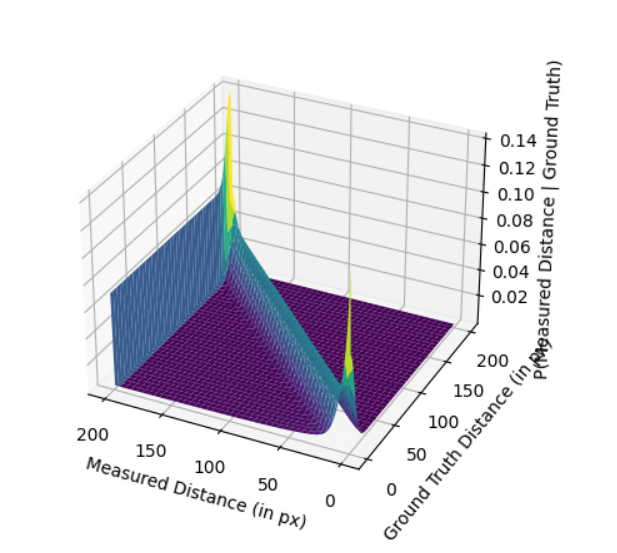
\includegraphics[scale=0.5]{figures/sensor_model_plot.png}
    \caption{Visualization of precomputed normalized probability table for a given measured distance, $z^{(i)}_k$, and ground truth, $d$.}
    \label{fig:1}
\end{figure}

With our probability template precomputed, retrieving the values based on our predicted sensor measurement and raycast ground truth values is significantly more efficient and faster.

\subsection{Particle Filter [Juan, Ningshan]}
    The particle filter combines the motion model and sensor model to calculate an estimated pose for the robot, as well as visualize the particle cloud in RVIZ. In the particle filter, we define several functions to allow for localization and particle generation. The function \texttt{odom\_callback} is responsible for transforming odometry data to updated hypothesis of localization. The function \texttt{laser\_callback} transforms laser data to updated probabilities of the robot's pose. Since both of them update the same class variables of self.particles of where the particles might be, threading is included to make sure no simultaneous editing happens on the particles. This is accomplished by adding locks and making sure the lock is acquired whenever changes happened on the variable and released when the process is completed.
    
   In more detail, we provide the robot with an initial pose in Rviz using the 2D pose estimate tool. This pose is communicated on the initial pose topic, but the message type contains the pose in 3 dimensions rather than the 2 dimensions needed by the other functions. To rectify this we implemented a \texttt{get\_2Dpose\_from\_3Dpose} function \texttt{odom\_callback} function reads in odometry data and uses the twist attribute of the \texttt{Odometry Message} type to find the velocity and \( d\theta \) of the robot, which is then fed into the motion model to determine the poses of the updated particles. These updated particles are then fed into the \texttt{laser\_callback} function, which uses the sensor model along with laser scan data to find the probabilities associated with each of the particles. During our tests we noticed that this approach caused our localization to converge extremely quickly on one pose, so in an effort to make the particles spread out, we raised the output of the probabilities to a fractional exponent. This operation causes the probabilities to be more uniform, preventing the model from fixating on one very high probability pose and resampling almost entirely based on that. The \texttt{publish\_array} function then generates a PoseArray and populates it with all the particles from the most recent resampling before publishing them to be visualized in Rviz. The function also generates an estimate of the robot's actual position based on the arithmetic mean of all of the particles' x and y positions, along with a circular mean of all of their yaw angles. A circular mean must be used in this case because an arithmetic mean would not provide the true average yaw angle for all of the particles. This estimated pose is then published alongside the particles as an odometry message. 


\section{Evaluation and Experimental Results [Erica, Ehab]}

First, we tested our MCL implementation in simulation with the car in wall following mode. We started with $100$ particles but noticed that the particles got very concentrated around some pose, so we took two measures to fix this:-

\begin{itemize}
    \item We increased the number of particles from $100$ to $1000$. The code was still running faster than $20$ Hz after that modification.
    \item We noticed only a few particles got a high probability and the rest got assigned a probability that is orders of magnitude lower, so we took the fourth roots of the estimated probabilities to make the distribution less peaked.
\end{itemize}

After these modifications, we could clearly see the particle cloud, and we achieved a very accurate result visually:-

\begin{figure}[H]
    \centering
    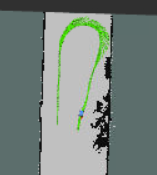
\includegraphics{RSS_localization.png}
    \caption{MCL result in simulation. The path from localization is shown in green, and the particle cloud is shown in red.}
    \label{fig:enter-label}
\end{figure}

We then evaluated the accuracy in simulation by comparing the ground truth position of the robot to the estimated pose. We graphed our x, y, and angle error over time in Figures 3, 4, and 5, respectively.

\begin{figure}[H]
    \centering
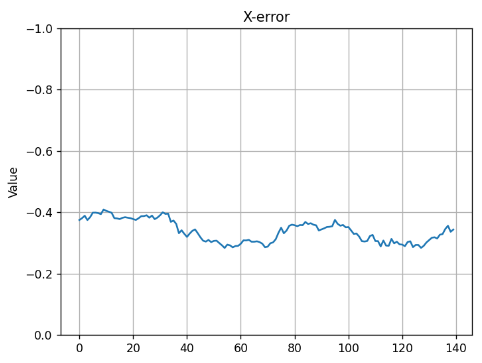
\includegraphics[scale=0.65]{figures/x_error.png}
    \caption{X-error of robot position in simulation. Average X-Error = 0.3382 m. We hypothesize that this X-Error includes the robot car length, which is 0.31 m. Accounting for that offset, we'd get a very small average error of 0.0282 m.}
    \label{fig:2}
\end{figure}

\begin{figure}[H]
    \centering
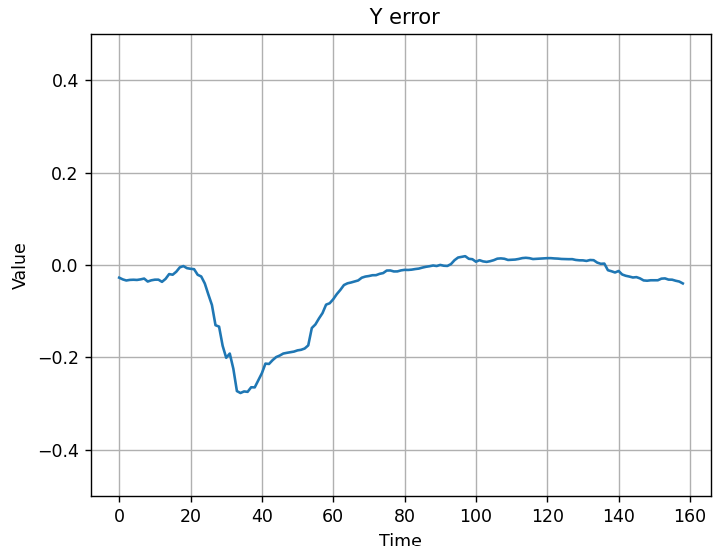
\includegraphics[scale=0.4]{figures/y_error.png}
    \caption{Y-error of robot position in simulation. Average Y-Error = -0.0494 m}
    \label{fig:3}
\end{figure}

\begin{figure}[H]
    \centering
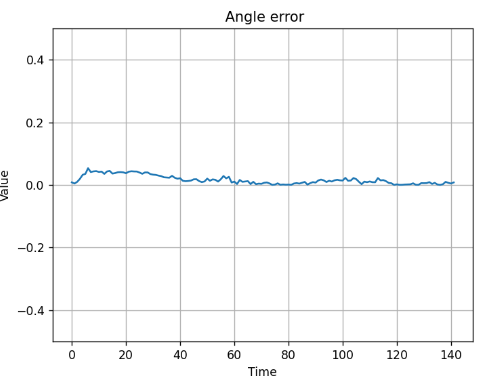
\includegraphics[scale=0.6]{figures/angle_error.png}
    \caption{Angle-error of robot position in simulation. Average Angle Error = 0.016 radians}
    \label{fig:4}
\end{figure}


For the evaluation of robot localization in real-life, we visually inspected it based on the known map in Stata basement. This is because in real-life, there is no ground-truth pose that we could easily compare it to while in motion. We placed the robot at a known position on the map, initialized its starting pose in simulation, and evaluated the accuracy of the particles clouds. We noticed the particle cloud was updating very slowly, so we decreased the number of particles back to $100$ to maintain a rate higher than $20$ Hz.

% The robot was successful at recovering its pose and odometry when stationary. However, we observe an inversion of the x-axis during the movement. When the robot is controlled to drive forward, the particle cloud in the simulation appears to be moving backward, resulting in an inaccurate localization in the map. To address this firmware setup error, we negated x, y, and $\theta$ when calculating particle pose in our motion model to accurately reflect the dynamic movement of the robot. Additionally, we fine tuned our motion model to set our velocity noise range to $0.3$ and our angle noise range to be $\frac{\pi}{30}$.

% After optimizing for real-life implementation, we tested and continued to fine tune our metrics for various turn angles and speeds. We graphed one such path that the robot was taking in Figure 6 and visually compared it to the actual motion of the robot.

After some parameter tuning, we managed to achieve accurate localization on the real car:-

\begin{figure}[H]
    \centering
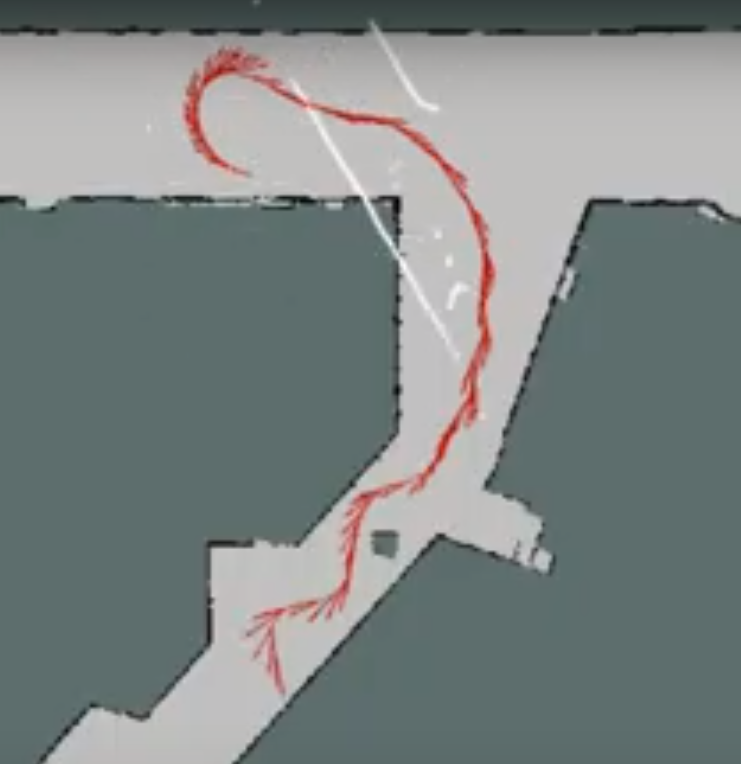
\includegraphics[scale=0.25]{figures/implementation_trail.png}
    \caption{Path of robot with varying speeds and angles. The trajectory shown was generated by \href{https://drive.google.com/file/d/13M48duxxxUkJKxFIRrq0tKB9kBgh_u8O/view?resourcekey}{this driving} and correlates visually well to the path the robot takes.}
    \label{fig:5}
\end{figure}

From visual inspection and correlation with a video of the robot motion, the estimated pose was accurate throughout various types of turns with intermittent and varying speeds. Ultimately, when amalgamated with our simulated errors, we were able to conclude that our simulation and tuned real-life implementation of MCL was sufficiently accurate. 

\section{Conclusions}

% In this lab, we investigated two localization techniques in robotics: the motion model and the sensor model. We adapted the Monte Carlo (MCL) approach to generate a batch of potential positions of the particles clouds, adding noise to provide robustness and flexibility. The particle candidates are then updated through the data received from the odometry of the robot and are updated as the robot moves in simulation. With more data coming from the sensor, the probabilities of each particle is assigned. 

% Through the sensor model that the calculations of probabilities are often too concentrated, leading to scenarios where certain localization hypotheses are assigned excessively high probabilities, while others receive disproportionately low probabilities. This lack of dispersion can hinder the model's ability to accurately represent the uncertainty inherent in the localization process. To broaden the distribution of probabilities, we raised the probability to the fourth root. This approach has allowed for a more comprehensive consideration of all potential localization hypotheses and effectively capturing the inherent uncertainty in the environment.

In conclusion, we managed to get an MCL implementation to work for both a simulated and real race car with reasonable accuracy.

We learned a few lessons as a team from this lab. For example, we learned that transitioning from simulation to reality presents unexpected challenges, such as limitations in hardware. We couldn't get the real racecar to work with nearly as many particles as in simulation. Furthermore, our racecar had a different convention for the axes than simulation, which made our particles move backwards when the robot was moving forwards until we detected and fixed it.

As for the communication component, what we learned as a group is to start the work early and communicate our progress in the lab in a timely fashion. 

Lessons learned by person:

\begin{itemize}
    \item Ningshan: The technical aspect I learned is to sample noise based on a normal distribution and can adjust the distribution by raising it to a root power. I also learned that it's very difficult to transfer the simulation to the stata basement because the actual basement has many objects that interfere with the LIDAR data and localization. For the communication component, I learned the lesson that we should document each progress we make by taking screenshots in a timely manner and compile the results before the presentation so we don't have the replicate our progress.
    \item Ehab: This lab taught me that I really ought to get better at delegating tasks. I'd started working on the lab earlier than the rest of the team and ended in a position where I had to be there for every little step of the development process, and ideally that shouldn't have been the case.
    \item Juan: This lab taught me a lot about how to represent a change in the position of a robot based on the odometry input. Forcing us to use twist instead of pose caused us to have to develop unique strategies for finding dx, dy, and dtheta that involved multiplying by the timesteps between function calls and taking the components of the velocity from twist. I also learned about the difficulties in transitioning from simulation to a real world environment, as multiple factors caused us to have to change the code to account for reality. For example, we had to flip the signs for our odometry updates due to hardware issues with the VESC, various objects placed around the Stata basement caused errors in our laser scan data, and we had to adjust the number of scans we took in to align with those used by the ray tracing code. For communication, I learned that it is important to have constant documentation of any tests done for material on reports and slides, and that we should communicate better as a team to finish communication assignments well before the due date. 
    \item Erica: Through this lab and other classes, I've encountered MCL, robot frames/motion models, discretization, Bayes filter, etc. However, it has always remained purely theoretical to me. Having actually applied it and seen it working step-by-step has given me a much better intuition of what each step actually represents. I've garnered a much better intuitive understanding of what these actually mean rather than seeing these steps (ie. Sensor Model) as only as vague equations. In terms of the communication side, I learned that if I don't understand something intuitively, asking multiple people's perspective may be beneficial. One person's picture of understanding may be more compatible with a certain thought process. Or by piecing together multiple snapshots of understanding, we're able to come together to form a clearer conceptual vision and understanding.
\end{itemize}

\end{document}